\RequirePackage[T1]{fontenc}
\documentclass[lettersize,journal]{IEEEtran}
\usepackage{amsmath,amssymb,graphicx,booktabs,array,cite}
\usepackage[hidelinks]{hyperref}
\usepackage{url}
\begin{document}
\title{Meta-AMS: Verified Multi-Seed Experimental Results and Statistical Audit}
\author{Meta-AMS Project\\Experimental Evidence Supplement---2 November 2026}
\maketitle

\begin{abstract}
This supplement reports the completed six-method comparison for a five-vehicle spatial lane-change task under hybrid attacks. All methods begin from one common real-trajectory behavior-cloning (BC) checkpoint and use three adaptation-training seeds, strict clean regression, and gated attack escalation. The executed campaign contains 104 training blocks, 4160 policy updates, 450 final evaluation records, and 162 final video evidence sets. Meta-AMS attains a hard-b whole-platoon completion mean of 93.06\%, with a sample standard deviation of 1.20 percentage points across training-seed means, and passes the hard-b gate in all three runs. Clean through hard-a completion is 100\%, and all recorded final evaluations have zero collision and road-boundary violation rates. These are conditional results of the implemented gated training and selection procedure. Early stopping, fallback to the common BC policy, differing realized budgets, and reuse of the evaluation seeds for selection are disclosed. Exploratory exact paired tests yield unadjusted two-sided $p=0.25$ and Holm-adjusted $p=1.00$ against each comparator; the present three-seed sample does not establish statistical significance.
\end{abstract}

\begin{IEEEkeywords}
Meta-AMS, multi-agent reinforcement learning, Ackermann platoon, reproducibility, training seeds, hybrid attacks.
\end{IEEEkeywords}

\section{Scope and Executed Protocol}
This report concerns only the campaign \texttt{ackermann\_completion\_20261027/uniform\_six}, completed on 2 November 2026 at 07:01 CST. It is distinct from the earlier single-chain comparison, the orthogonal-ablation cohort, and the repaired retention-continuation cohort. Their numerical results are not pooled. The original manuscript's algorithmic propositions are not rederived or modified here.

\subsection{Common Initialization and Task}
Each method starts from the same supplied BC checkpoint, fitted using simulator-executed vehicle trajectories. The adaptation seeds are 42, 3407, and 777. These are three adaptation runs conditional on one BC fit, not three independent BC fits or three runs from random initialization. The task uses five simulated Ackermann vehicles following one spatial lane-change path, with front steering and no rear steering in the recorded vehicle interface. The initial vehicle spacing is 1.50 m; the shared spatial transition starts at $x=-7.75$ m and has length 6 m, connecting $y=-0.065$ m to $y=-1.160$ m.

Every reported final evaluation uses 16 environments and 3500 steps (70 s). Each attacked checkpoint is evaluated at the fixed environment/attack seed pairs $(42,3407)$, $(3407,9917)$, and $(777,17011)$. Clean evaluation uses $(42,3407)$. The same pairs are also used during candidate promotion. Thus, the final matrices are selected-policy assessments on fixed evaluation conditions, not a separate held-out generalization test.

\subsection{Completion, Safety, and Promotion}
The reported completion is the fraction of environments in which the entire five-vehicle platoon has satisfied the implemented completion conditions with the required 2 s dwell at least once within the evaluation horizon. The recorded tolerances include path progress at least 0.99, lateral error at most 0.12 m, heading error at most 0.12 rad, gap error at most 0.35 m, and pair lateral error at most 0.20 m. Cumulative completion is not the fraction continuously satisfying the conditions for the entire episode or after the terminal reset.

Strict clean acceptance requires cumulative completion, peak instantaneous completion and peak dwell completion all equal to one, with zero collision, road-boundary-any violation and road-boundary termination. Attack promotion additionally uses the minimum completion across all three evaluation pairs. Its thresholds are 0.75 for light through easy-b, 0.65 for med-a, 0.55 for med-b, and 0.50 for hard-a and hard-b. Safety requirements remain zero throughout.

\subsection{Training and Method Identity}
The campaign uses 32 training environments, 32 rollout steps per update, a cap of 40 updates per attack stage, and one candidate per stage. Eight successful attack stages therefore correspond to 320 updates. The actor learning rate is $5\times10^{-7}$. The BC and reference-policy KL coefficients are 4.0 and 0.8. Expert action blending and retention/expert-exit schedules are disabled during this campaign; the safety shield remains active. Training mixes 50\% clean environments with the configured attack profile at full stage strength. Evaluation uses full attack strength and no clean mixture.

The AMS configuration uses $K=8$, normalized radius 0.25, maximum advantage weight 0.1, 50-update warm-up and 100-update ramp, and risk coefficient zero. These are configuration values, not empirical evidence for the theoretical isotropy or smoothness assumptions. Table~\ref{tab:methods} records the actual method switches. Different actor-sharing and update rules prevent attributing every six-method difference solely to AMS or the meta teacher.
\begin{table}[t]
\centering
\caption{Method switches in the executed repository implementations.}
\label{tab:methods}
\small
\setlength{\tabcolsep}{4pt}
\begin{tabular}{lrrrrl}
\toprule
Method & Meta & AMS & Factor & Shared & Update \\
\midrule
MAPPO & 0 & 0 & 0 & 0 & PPO \\
HAPPO (no Meta) & 0 & 0 & 1 & 0 & PPO \\
Meta-AMS & 1 & 1 & 1 & 1 & PPO \\
Shared MAPPO & 0 & 0 & 0 & 1 & PPO \\
HAA2C & 0 & 0 & 1 & 1 & A2C \\
HATRPO & 0 & 0 & 1 & 1 & TRPO \\
\bottomrule
\end{tabular}

\vspace{2pt}\begin{minipage}{\linewidth}\footnotesize These are the repository implementations selected by the recorded flags, not a claim of unmodified external HARL code. Architecture/sharing differs between some rows.\end{minipage}
\end{table}


\section{Completed Results}
All 18 method--training-seed procedures reached a recorded terminal outcome under the fixed gate rules. This means the prescribed comparison is complete, not that all methods successfully trained through hard-b. Every final retained model was assessed at clean and all eight attack strengths. The final evidence comprises $18(1+8\times3)=450$ evaluation records and $18\times9=162$ video/trajectory evidence sets.

\begin{table}[t]
\centering
\caption{Final retained policies at hard-b: completion in percent.}
\label{tab:hardb}
\small
\setlength{\tabcolsep}{4pt}
\begin{tabular}{lrrr}
\toprule
Method & Mean $\pm$ SD & Worst & Pass \\
\midrule
MAPPO & 46.53 $\pm$ 2.41 & 37.50 & 0/3 \\
HAPPO (no Meta) & 47.22 $\pm$ 7.89 & 37.50 & 1/3 \\
Meta-AMS & 93.06 $\pm$ 1.20 & 87.50 & 3/3 \\
Shared MAPPO & 2.78 $\pm$ 4.81 & 0.00 & 0/3 \\
HAA2C & 27.08 $\pm$ 20.52 & 6.25 & 0/3 \\
HATRPO & 0.00 $\pm$ 0.00 & 0.00 & 0/3 \\
\bottomrule
\end{tabular}

\vspace{2pt}\begin{minipage}{\linewidth}\footnotesize SD is across three training-seed means, not nine independent fits. Pass counts final evaluation gates. HATRPO retains the common BC model in all three runs; shared MAPPO does so in two runs.\end{minipage}
\end{table}

\begin{table*}[t]
\centering
\caption{Mean whole-platoon completion (percent) across the complete ladder.}
\label{tab:ladder}
\small
\setlength{\tabcolsep}{4pt}
\begin{tabular}{lrrrrrrrrr}
\toprule
Method & off & light & easy\_0 & easy\_a & easy\_b & med\_a & med\_b & hard\_a & hard\_b \\
\midrule
MAPPO & 100.00 & 100.00 & 100.00 & 100.00 & 100.00 & 100.00 & 100.00 & 95.14 & 46.53 \\
HAPPO (no Meta) & 100.00 & 100.00 & 100.00 & 100.00 & 100.00 & 100.00 & 100.00 & 95.83 & 47.22 \\
Meta-AMS & 100.00 & 100.00 & 100.00 & 100.00 & 100.00 & 100.00 & 100.00 & 100.00 & 93.06 \\
Shared MAPPO & 100.00 & 59.72 & 43.06 & 45.83 & 37.50 & 38.89 & 35.42 & 25.00 & 2.78 \\
HAA2C & 100.00 & 100.00 & 100.00 & 97.22 & 93.06 & 81.94 & 83.33 & 65.97 & 27.08 \\
HATRPO & 100.00 & 39.58 & 14.58 & 18.75 & 6.25 & 14.58 & 10.42 & 10.42 & 0.00 \\
\bottomrule
\end{tabular}

\vspace{2pt}\begin{minipage}{\linewidth}\footnotesize Each attack cell averages three training-seed means, each obtained from three fixed environment/attack seed pairs. The clean cell uses one evaluation pair per training seed.\end{minipage}
\end{table*}


\subsection{Meta-AMS}
Meta-AMS passes all training-stage gates in all three runs. Its final hard-b training-seed means are 93.75\%, 93.75\%, and 91.67\%. Their overall mean is 93.06\%; the sample standard deviation is 1.20 percentage points. The worst of the nine hard-b evaluation records is 87.5\%. Clean through hard-a completion is 100\% in all three training runs and all corresponding evaluation pairs. All 450 final evaluations, including the baselines, have zero recorded collision, road-boundary-any violation and road-boundary termination. Safety without maneuver completion is not counted as task success.

\begin{figure*}[t]
\centering
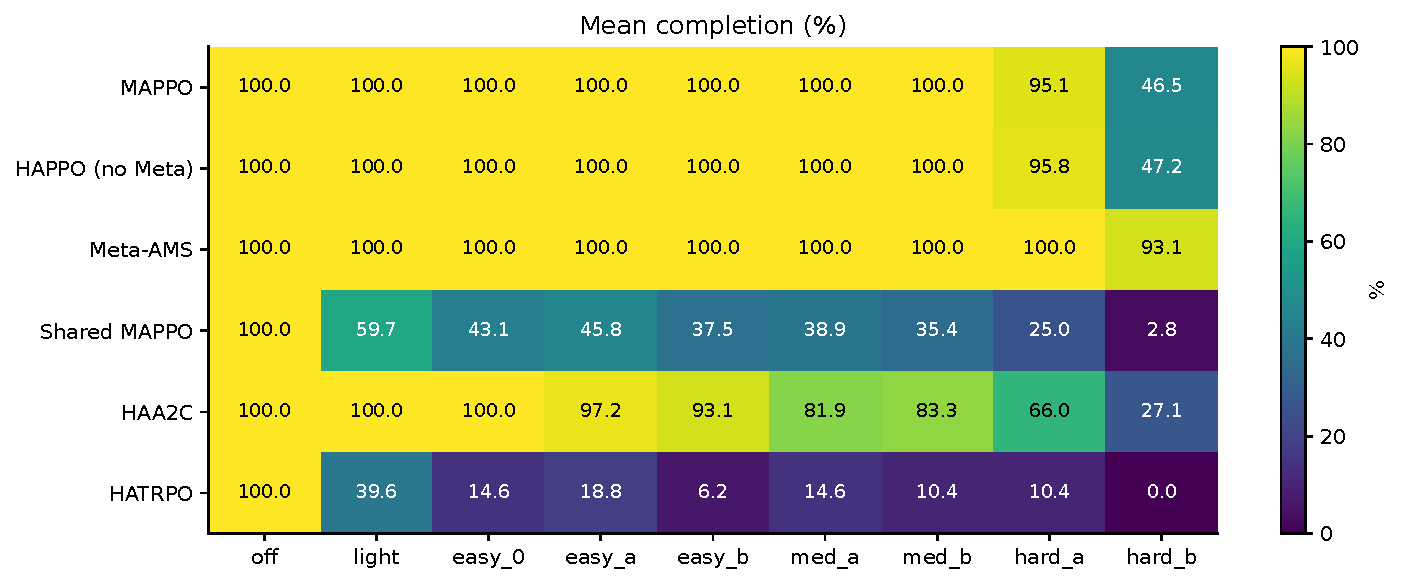
\includegraphics[width=.96\textwidth]{figures/completion_mean.pdf}
\caption{Full-ladder mean completion. Each attacked cell first averages the three evaluation pairs within each adaptation seed, then averages the three adaptation-seed means. Early-stopped methods retain their last accepted model.}
\label{fig:matrix}
\end{figure*}

\begin{figure*}[t]
\centering
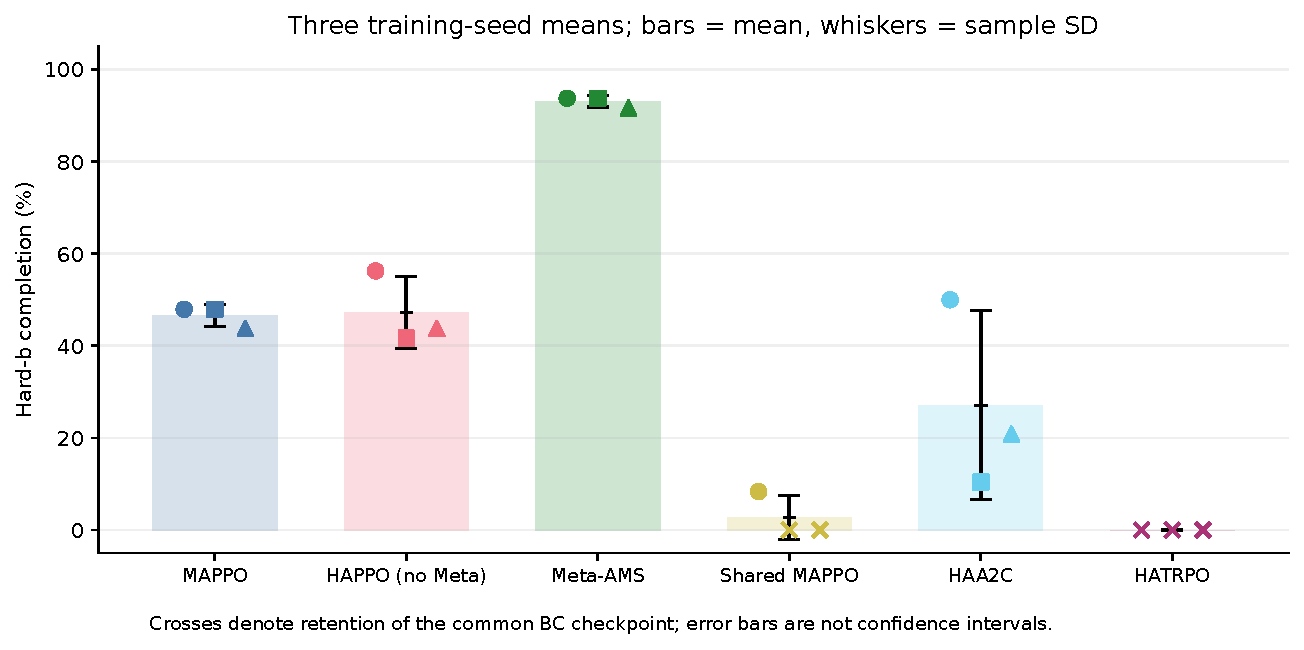
\includegraphics[width=.94\textwidth]{figures/hard_b_training_seeds.pdf}
\caption{Hard-b results with all three training-seed means visible. Whiskers are sample standard deviations, not confidence intervals. Crosses identify fallback to the common BC checkpoint; repeated fallback values must not be described as distinct successfully trained policies.}
\label{fig:seeds}
\end{figure*}

\subsection{Retained Policies and Rejected Candidates}
The tables use the final \emph{retained} checkpoint. A rejected hard-b candidate is not substituted into the final comparison. For example, HAPPO without Meta stops at a rejected hard-b candidate in every run and retains its hard-a checkpoint. The retained s0 checkpoint subsequently passes the hard-b assessment (minimum 50\%), even though its newer hard-b candidate had failed. These are different checkpoints, not contradictory evaluations of one model.

The three HATRPO candidates all fail the clean regression after their first light-stage training block and fall back to the same BC checkpoint. Shared MAPPO does so in s1 and s2. Consequently, the retained checkpoint counts are three for MAPPO, HAPPO without Meta, Meta-AMS and HAA2C, two for shared MAPPO, and one for HATRPO. The zero hard-b results for HATRPO describe that common fallback policy after unsuccessful training attempts; they do not show three independently trained HATRPO policies with zero variance.

\begin{table*}[t]
\centering
\caption{Realized training budgets and retained stages.}
\label{tab:budget}
\small
\setlength{\tabcolsep}{4pt}
\begin{tabular}{lrrrlr}
\toprule
Method & s0 A/R & s1 A/R & s2 A/R & Retained stage s0/s1/s2 & BC \\
\midrule
MAPPO & 320/280 & 320/280 & 320/280 & hard\_a/hard\_a/hard\_a & 0 \\
HAPPO (no Meta) & 320/280 & 320/280 & 320/280 & hard\_a/hard\_a/hard\_a & 0 \\
Meta-AMS & 320/320 & 320/320 & 320/320 & hard\_b/hard\_b/hard\_b & 0 \\
Shared MAPPO & 320/280 & 40/0 & 40/0 & hard\_a/BC/BC & 2 \\
HAA2C & 320/280 & 160/120 & 280/240 & hard\_a/easy\_a/med\_b & 0 \\
HATRPO & 40/0 & 40/0 & 40/0 & BC/BC/BC & 3 \\
\bottomrule
\end{tabular}

\vspace{2pt}\begin{minipage}{\linewidth}\footnotesize A: attempted updates, including rejected candidates; R: updates on the retained lineage. BC: number of runs retaining the common warm start. Each block uses 40 updates, 32 environments and 32 rollout steps per update. Equal per-stage caps do not imply equal realized budgets or equal wall-clock computation.\end{minipage}
\end{table*}

Table~\ref{tab:budget} discloses both attempted and retained training updates. Total attempted updates are 4160, corresponding to 4,259,840 recorded environment transitions. This total excludes the shared BC fit, all evaluations, and video recording. The campaign equalizes the per-stage cap and promotion criteria; realized training budgets differ because of early stopping. It therefore compares the executed training-and-selection procedures, not fully tuned algorithms under equal total compute.

\section{Training-Seed Statistical Analysis}
\subsection{Unit of Analysis}
For method $m$, adaptation seed $s$, and hard-b evaluation pair $e$, let $C_{mse}$ be the recorded whole-platoon completion rate. We first compute
\begin{equation}
M_{ms}=\frac{1}{3}\sum_{e=1}^{3}C_{mse},\qquad
\widehat{\mu}_m=\frac{1}{3}\sum_{s=1}^{3}M_{ms}.
\end{equation}
The descriptive spread is the sample standard deviation of the three $M_{ms}$ values, using denominator $3-1$. The nine evaluations, the 16 parallel environments, the five vehicles, and the 3500 time steps are not substituted for independent training replicates. We report raw seed points and SD, rather than presenting a small-sample bootstrap interval as a reliable population confidence interval.

\subsection{Exploratory Exact Paired Tests}
Hard-b is the exploratory endpoint for the five Meta-AMS versus comparator contrasts. This analysis was defined after the results were available; it is not preregistered. Matching uses the common adaptation-seed index. Let $D_s=M_{\mathrm{Meta\text{-}AMS},s}-M_{m,s}$ and $T=|\frac{1}{3}\sum_s D_s|$. We enumerate all $2^3=8$ sign assignments $\boldsymbol\eta\in\{-1,+1\}^3$ and compute
\begin{equation}
p_m=\frac{1}{8}\sum_{\boldsymbol\eta}
\mathbf{1}\!\left\{\left|\frac{1}{3}\sum_{s=1}^{3}\eta_sD_s\right|\geq T\right\}.
\end{equation}
This is the two-sided paired sample-label/sign-flip construction described in the permutation-test documentation \cite{scipyperm}. Its conditional validity requires exchangeability of the paired labels/signs under the null, and independence across seed pairs conditional on the common fixed BC fit. Matching the integer seed alone does not prove these assumptions. The estimand includes the deterministic gate, selection and fallback rule. It is not the performance of a successfully trained policy conditional on surviving selection.

\begin{table}[t]
\centering
\caption{Exploratory paired hard-b comparisons: Meta-AMS minus comparator.}
\label{tab:tests}
\small
\setlength{\tabcolsep}{4pt}
\begin{tabular}{lrrr}
\toprule
Comparator & $\Delta$ (pp) & Exact $p$ & Holm $p$ \\
\midrule
MAPPO & 46.53 & 0.25 & 1.00 \\
HAPPO (no Meta) & 45.83 & 0.25 & 1.00 \\
Shared MAPPO & 90.28 & 0.25 & 1.00 \\
HAA2C & 65.97 & 0.25 & 1.00 \\
HATRPO & 93.06 & 0.25 & 1.00 \\
\bottomrule
\end{tabular}

\vspace{2pt}\begin{minipage}{\linewidth}\footnotesize Two-sided exact sign-flip tests enumerate all eight sign assignments of three matched seed differences. Five post-hoc comparisons form one Holm family. This tests the gated procedure conditional on exchangeability; it does not isolate an AMS module effect.\end{minipage}
\end{table}


Every observed paired difference is positive, but each contrast still has $p=2/8=0.25$: both the all-positive and all-negative assignments are equally extreme. Holm correction across the five comparisons \cite{holmimplementation} yields adjusted $p=1.00$ for each. No contrast rejects at $\alpha=0.05$. This is limited statistical resolution, not evidence that the observed effect sizes are zero. We therefore use ``higher observed completion under this protocol,'' not ``statistically significant superiority.'' No favorable one-sided alternative was selected after observing the signs.

The eight-assignment distribution for every contrast is included as a CSV. As a resolution calculation only, with five comparisons the first Holm threshold is $0.05/5=0.01$; $2/2^n$ can reach it only when $n\geq8$. This is not a power calculation or a guarantee that eight future seeds would establish significance. New runs would also need a fixed analysis plan and a clear decision about independent BC initialization and held-out evaluation conditions.

\section{Trajectory and Learning-Curve Evidence}
The example in Fig.~\ref{fig:path} is the recorded s0 hard-b rendered rollout, selected by a fixed rule rather than the best observed completion. Its original 70 s video and all 17,500 vehicle/time rows are included. It is a one-environment rendering and is distinct from the 16-environment numerical assessments. Individual paths and progress traces illustrate sequential traversal of the common spatial maneuver; aggregate completion and safety claims come from the separate verified evaluation records. The final reset discontinuity is omitted only from the continuous path drawing; the raw CSV and video are preserved.

\begin{figure}[t]
\centering
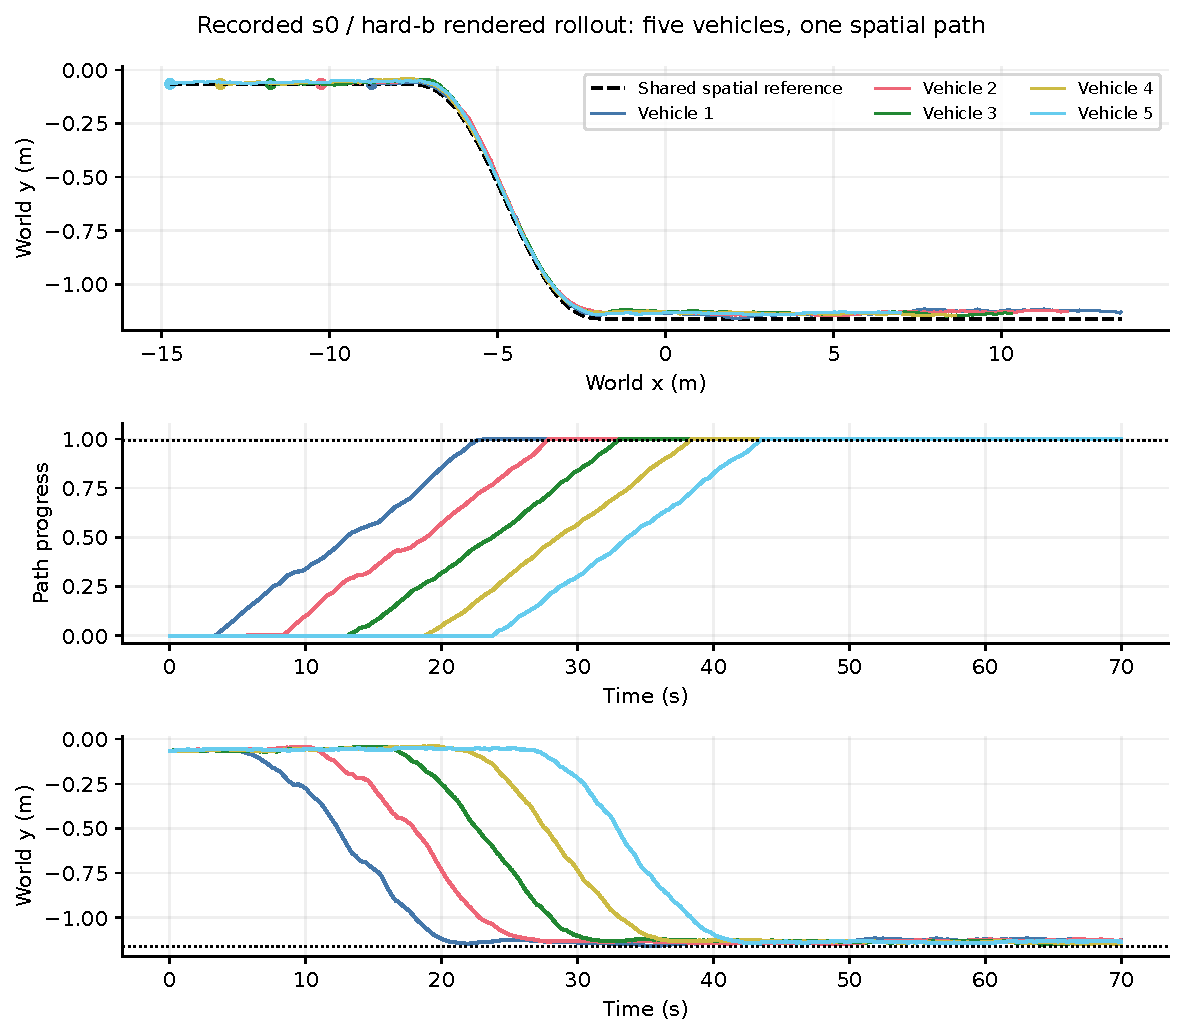
\includegraphics[width=\columnwidth]{figures/five_vehicle_lane_change.pdf}
\caption{Recorded five-vehicle maneuver in the representative s0 hard-b rendering. The spatial reference and each vehicle's own path progress distinguish sequential path following from imposing simultaneous lateral positions. This illustrative rollout is not an additional independent evaluation seed.}
\label{fig:path}
\end{figure}

\begin{figure*}[t]
\centering
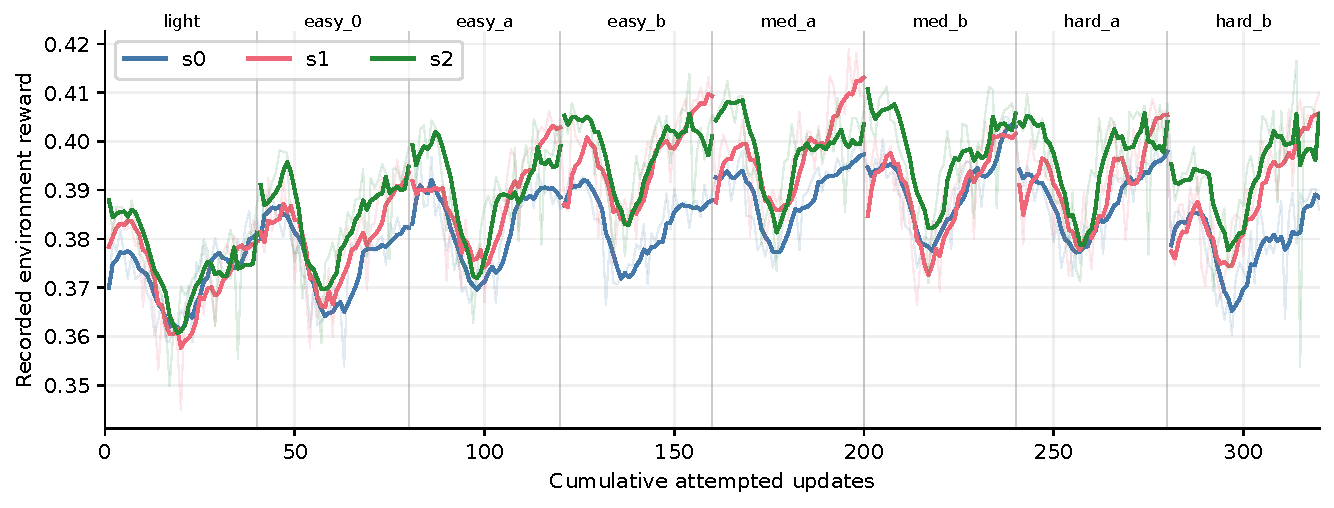
\includegraphics[width=.96\textwidth]{figures/meta_ams_training_reward.pdf}
\caption{Recorded Meta-AMS environment rewards for the three adaptation seeds. Thin curves are update samples; thick curves are five-update rolling means computed separately within each stage. Attack budgets change at stage boundaries, so the trace is descriptive and does not represent one stationary learning objective.}
\label{fig:rewards}
\end{figure*}

\section{Paper Integration and Remaining Evidence Boundaries}
The new six-method data support the combined implemented method under the disclosed shared-BC, shield-enabled, gated protocol. They do not isolate the causal interaction of Meta and AMS: the six rows include different sharing and update choices. A matched $2\times2$ ablation belongs to a separate cohort and must not be silently merged with this one. Likewise, BC/KL retention is enabled across this comparison and there is no contemporaneous no-retention control; this matrix alone cannot establish a causal retention benefit or a guarantee against forgetting.

The experiment uses one simulator scenario, fixed evaluation pairs, one BC fit and only three adaptation seeds. Its clean and attack thresholds were not relaxed, but evaluation-conditioned selection limits a held-out robustness interpretation. Zero observed safety violations are empirical outcomes under the active shield, not a formal safety guarantee or a validation of Proposition 1.

For the main manuscript, the new results should update the abstract, contribution/result statements, full-ladder tables, six-method comparison, limitations and conclusion together. The old 75\% single-chain figure and the separate 90.28\% repaired-continuation average must retain their original cohort labels if discussed. The main manuscript's AMS equations, projection definition and smoothness assumptions require their own code/formula audit and are not repaired by changing the experimental tables. An accompanying Chinese integration note lists the specific source locations.

\section{Reproducibility}
The package contains portable per-evaluation metrics, per-stage training budgets, all selected checkpoint identities, exact permutation distributions, generated LaTeX tables, PDF/PNG figures, the campaign's hash-verified source snapshot, and the representative original video. All 450 original evaluation summaries and verification manifests are included. The much larger complete per-step CSVs, all 162 videos and checkpoints remain at the server paths recorded in the input manifest; this supplement is not a replacement for that full raw archive.

\noindent Rebuild the numerical tables and plots with:\\
{\footnotesize\ttfamily python scripts/build\_ackermann\_paper\_results.py\\
--output . --rebuild}

The data originate from the recorded completed queue. No new training or simulation was run for this supplement. The final systemd timeout flag occurred during cleanup of a telemetry subprocess after the main process had exited successfully; independent artifact checks verified the completed results.

\bibliographystyle{IEEEtran}
\bibliography{references/statistical_methods}
\end{document}
